
\chapter{Portfolio Construction}
\label{chap:portfolio}
\lhead{Chapter 3. \emph{Portfolio Construction}}

In the introduction, we discussed how relaxing the Gaussian assumption often sacrifices analytical clarity or leads to intractable estimation. By contrast, our GMM and KDE frameworks can capture skewness and heavy tails without giving up closed-form interpretability. This chapter builds on the classical mean-variance paradigm by combining our density estimators with exponential utility maximization. The resultant portfolios incorporate information about higher moments of asset returns yet retain the tractability of Markowitz's original approach.

\section{Modeling Returns}
Let $\mathbf{r}$ represent a random vector of asset returns in $\mathbb{R}^{d}$, where $d$ is the number of assets. We observe a time series of $n$ return realizations, denoted as
$$\mathbf{r}_{1},\mathbf{r}_2,...,\mathbf{r}_{n}\quad\text{where}\quad \mathbf{r}_{\it{i}}\in\mathbb{R}^{d}.$$

The portfolio return is defined as the scalar random variable
$$R(\mathbf{w})=\mathbf{w}^{\mathsf{T}}\mathbf{r},$$
where $\mathbf{w}\in\mathbb{R}^{d}$ is the vector of portfolio weights. Under exponential utility, the investor has the utility function
$$U(R(\mathbf{w}))=-\exp(-\gamma\mathbf{w}^{\mathsf{T}}\mathbf{r}),$$
with $\gamma$ is the risk aversion parameter.

Both KDE and GMM estimate the density of $\mathbf{r}\rightarrow\hat{f}(\mathbf{r})$, enabling us to compute the expected utility of the portfolio return:
$$\mathbb{E}[U(R(\mathbf{w}))]=\int_{\mathbb{R}^{d}}-\exp(-\gamma\mathbf{w}^{\mathsf{T}}\mathbf{r})\cdot\hat{f}(\mathbf{r})\,d\mathbf{r}$$

Since both KDE and GMM approximate the density as a weighted sum of Gaussian components, 
we can compute the overall expected utility as the weighted sum of expectations over each density component.

Now we recall the KD estimator: 
$$\displaystyle\hat{f_h}(\mathbf{x})=\frac{1}{n}\sum_{i=1}^{n}K_\mathbf{H}(\mathbf{x}-\mathbf{x}_i),$$
for which when Gaussian kernel is used, $K_\mathbf{H}$ can be written as
$$K_\mathbf{H}(\mathbf{r}-\mathbf{r}_i)=\mathcal{N}(\mathbf{r|r_{\it{i}},H}).$$

Additionally, we recall the known result for Gaussian expectations:
$$\mathbb{E}_{\mathbf{r}\sim\mathcal{N}(\mathbf{\mu,\Sigma})}[\exp(-\gamma\mathbf{w}^{\mathsf{T}}\mathbf{r})]=\exp\left(-\gamma\mathbf{w}^{\mathsf{T}}\mathbf{\mu}+\frac{1}{2}\gamma^2\mathbf{w}^{\mathsf{T}}\mathbf{\Sigma}\mathbf{w}\right)$$

Having established the above, we take the expectation under GMM and KDE side by side to demonstrate their similarity:
$$GMM:\qquad\mathbb{E}[U(R(\mathbf{w}))]=\int_{\mathbb{R}^{d}}-\exp(-\gamma\mathbf{w}^{\mathsf{T}}\mathbf{r})\cdot\sum_{i=1}^{K}\phi_{i} \mathcal{N}(\mathbf{r|\mu_{\it{i}},\Sigma_{\it{i}}})\,d\mathbf{r}$$

$$\,KDE:\qquad\mathbb{E}[U(R(\mathbf{w}))]=\int_{\mathbb{R}^{d}}-\exp(-\gamma\mathbf{w}^{\mathsf{T}}\mathbf{r})\cdot \sum_{i=1}^{n}\frac{1}{n}\mathcal{N}(\mathbf{r|r_{\it{i}},H})\,d\mathbf{r}\,$$

Which, by linearity, is equivalent to:
$$GMM:\qquad=-\sum_{i=1}^{K}\phi_{i}\int_{\mathbb{R}^{d}}\exp(-\gamma\mathbf{w}^{\mathsf{T}}\mathbf{r})\cdot \mathcal{N}(\mathbf{r|\mu_{\it{i}},\Sigma_{\it{i}}})\,d\mathbf{r}$$

$$\,KDE:\qquad=-\frac{1}{n}\sum_{i=1}^{n}\int_{\mathbb{R}^{d}}\exp(-\gamma\mathbf{w}^{\mathsf{T}}\mathbf{r})\cdot \mathcal{N}(\mathbf{r|r_{\it{i}},H})\,d\mathbf{r}\,\,\,$$

Substituting the normal density:
$$GMM:\qquad=-\sum_{i=1}^{K}\phi_{i}\int_{\mathbb{R}^{d}}\exp(-\gamma\mathbf{w}^{\mathsf{T}}\mathbf{r})\cdot \frac{1}{(2\pi)^{d/2}\sqrt{\det{(\mathbf{\Sigma_{\it{i}}})}}}\exp\left(-\frac{1}{2}\mathbf{(r-\mu_{\it{i}})^\mathsf{T}\Sigma_{\it{i}}^\mathrm{-1}(r-\mu_{\it{i}})}\right)d\mathbf{r}\,$$

$$\,KDE:\qquad\displaystyle=-\frac{1}{n}\sum_{i=1}^{n}\int_{\mathbb{R}^{d}}\exp(-\gamma\mathbf{w}^{\mathsf{T}}\mathbf{r})\cdot\frac{1}{(2\pi)^{d/2}\sqrt{\det{(\mathbf{H})}}}\exp\left(-\frac{1}{2}\mathbf{(r-r_{\it{i}})^\mathsf{T}H^\mathrm{-1}(r-r_{\it{i}})}\right)d\mathbf{r}\,$$

Finally, by applying the Gaussian expectation, we obtain:
$$GMM:\qquad\mathbb{E}[U(R(\mathbf{w}))]=-\sum_{i=1}^{K}\phi_{i}\exp\left(-\gamma\mathbf{w}^{\mathsf{T}}\mathbf{\mu}_i+\frac{1}{2}\gamma^2\mathbf{w}^{\mathsf{T}}\mathbf{\Sigma}_i\mathbf{w}\right)$$

$$\qquad\quad\equiv-\sum_{i=1}^{K}\phi_{i}\mathbb{E}_{i}[U(R(\mathbf{w}))]$$

Where $\mathbb{E}_{i}[U(R(\mathbf{w}))]$ is the expected utility for each of the $K$ Gaussian kernels.
$$\,KDE:\qquad\mathbb{E}[U(R(\mathbf{w}))]=-\frac{1}{n}\sum_{i=1}^{n}\exp\left(-\gamma\mathbf{w}^{\mathsf{T}}\mathbf{r}_i+\frac{1}{2}\gamma^2\mathbf{w}^{\mathsf{T}}\mathbf{H}\mathbf{w}\right)$$
$$\qquad\qquad\qquad\qquad\qquad\qquad\,\,=-\frac{1}{n}\exp\left(\frac{1}{2}\gamma^2\mathbf{w}^{\mathsf{T}}\mathbf{H}\mathbf{w}\right)\sum_{i=1}^{n}\exp\left(-\gamma\mathbf{w}^{\mathsf{T}}\mathbf{r}_i\right)$$


\section{Portfolio Construction}
\subsection{GMM Portfolio}
Having derived exact expressions for $\mathbb{E}[U(R(\mathbf w))]$ under each return model, all that is left is the choice of the optimal $\mathbf w$. We begin by maximizing the expected utility:

\begin{align*}
\arg\max_\mathbf{w}{\mathbb{E}[U(R(\mathbf{w}))]} &= \arg\max_\mathbf{w}{-\sum_{i=1}^{K}\phi_{i}\exp\left(-\gamma\mathbf{w}^{\mathsf{T}}\mathbf{\mu}_i+\frac{1}{2}\gamma^2\mathbf{w}^{\mathsf{T}}\mathbf{\Sigma}_i\mathbf{w}\right)} \\
\intertext{Since multiplying by -1 flips the maximization into minimization, we rewrite the objective as}
&= \arg\min_\mathbf{w}{\sum_{i=1}^{K}\phi_{i}\exp\left(-\gamma\mathbf{w}^{\mathsf{T}}\mathbf{\mu}_i+\frac{1}{2}\gamma^2\mathbf{w}^{\mathsf{T}}\mathbf{\Sigma}_i\mathbf{w}\right)} \\
\intertext{To simplify the exponential sum and exploit convexity, we apply the monotonic logarithm, yielding}
&= \arg\min_\mathbf{w}\log{\left[{\sum_{i=1}^{K}\phi_{i}\exp\left(-\gamma\mathbf{w}^{\mathsf{T}}\mathbf{\mu}_i+\frac{1}{2}\gamma^2\mathbf{w}^{\mathsf{T}}\mathbf{\Sigma}_i\mathbf{w}\right)}\right]} \\
\intertext{Factoring out the component weights inside the exponent gives}
&= \arg\min_\mathbf{w}\log{\left[{\sum_{i=1}^{K}\exp({\log{\phi_{i}}})\exp\left(-\gamma\mathbf{w}^{\mathsf{T}}\mathbf{\mu}_i+\frac{1}{2}\gamma^2\mathbf{w}^{\mathsf{T}}\mathbf{\Sigma}_i\mathbf{w}\right)}\right]} \\
&= \arg\min_\mathbf{w}\log{\left[{\sum_{i=1}^{K}\exp\left(\log{\phi_{i}}-\gamma\mathbf{w}^{\mathsf{T}}\mathbf{\mu}_i+\frac{1}{2}\gamma^2\mathbf{w}^{\mathsf{T}}\mathbf{\Sigma}_i\mathbf{w}\right)}\right]} \\
\intertext{Recognizing this as the log-sum-exp operator (LSE), we obtain the compact form}
&= \arg\min_\mathbf{w}LSE_i\left(\log{\phi_{i}}-\gamma\mathbf{w}^{\mathsf{T}}\mathbf{\mu}_i+\frac{1}{2}\gamma^2\mathbf{w}^{\mathsf{T}}\mathbf{\Sigma}_i\mathbf{w}\right)
\end{align*}

% Having derived exact expressions for $\mathbb{E}[U(R(\mathbf w))]$ under each return model, all that is left is the choice of the optimal $\mathbf w$. We begin by maximizing the expected utility:
% $$\arg\max_\mathbf{w}{\mathbb{E}[U(R(\mathbf{w}))]}=\arg\max_\mathbf{w}{-\sum_{i=1}^{K}\phi_{i}\exp\left(-\gamma\mathbf{w}^{\mathsf{T}}\mathbf{\mu}_i+\frac{1}{2}\gamma^2\mathbf{w}^{\mathsf{T}}\mathbf{\Sigma}_i\mathbf{w}\right)}$$

% Since multiplying by -1 flips the maximization into minimization, we rewrite the objective as
% $$=\arg\min_\mathbf{w}{\sum_{i=1}^{K}\phi_{i}\exp\left(-\gamma\mathbf{w}^{\mathsf{T}}\mathbf{\mu}_i+\frac{1}{2}\gamma^2\mathbf{w}^{\mathsf{T}}\mathbf{\Sigma}_i\mathbf{w}\right)}$$

% To simplify the exponential sum and exploit convexity, we apply the monotonic logarithm, yielding
% $$=\arg\min_\mathbf{w}\log{\left[{\sum_{i=1}^{K}\phi_{i}\exp\left(-\gamma\mathbf{w}^{\mathsf{T}}\mathbf{\mu}_i+\frac{1}{2}\gamma^2\mathbf{w}^{\mathsf{T}}\mathbf{\Sigma}_i\mathbf{w}\right)}\right]}$$

% Factoring out the component weights inside the exponent gives
% $$=\arg\min_\mathbf{w}\log{\left[{\sum_{i=1}^{K}\exp({\log{\phi_{i}}})\exp\left(-\gamma\mathbf{w}^{\mathsf{T}}\mathbf{\mu}_i+\frac{1}{2}\gamma^2\mathbf{w}^{\mathsf{T}}\mathbf{\Sigma}_i\mathbf{w}\right)}\right]}$$

% $$=\arg\min_\mathbf{w}\log{\left[{\sum_{i=1}^{K}\exp\left(\log{\phi_{i}}-\gamma\mathbf{w}^{\mathsf{T}}\mathbf{\mu}_i+\frac{1}{2}\gamma^2\mathbf{w}^{\mathsf{T}}\mathbf{\Sigma}_i\mathbf{w}\right)}\right]}$$

% Recognizing this as the log-sum-exp operator (LSE), we obtain the compact form
% $$=\arg\min_\mathbf{w}LSE_i\left(\log{\phi_{i}}-\gamma\mathbf{w}^{\mathsf{T}}\mathbf{\mu}_i+\frac{1}{2}\gamma^2\mathbf{w}^{\mathsf{T}}\mathbf{\Sigma}_i\mathbf{w}\right)$$

Setting up Lagrangian and imposing the fully invested constraint:
$$\mathcal{L}=LSE_i\left(\log{\phi_{i}}-\gamma\mathbf{w}^{\mathsf{T}}\mathbf{\mu}_i+\frac{1}{2}\gamma^2\mathbf{w}^{\mathsf{T}}\mathbf{\Sigma}_i\mathbf{w}\right)+\lambda(\mathbf{w^{\mathsf{T}}1}-1)$$

For notational simplicity, let us define
$$f_i(\mathbf{w})=\log{\phi_{i}}-\gamma\mathbf{w}^{\mathsf{T}}\mathbf{\mu}_i+\frac{1}{2}\gamma^2\mathbf{w}^{\mathsf{T}}\mathbf{\Sigma}_i\mathbf{w}$$
$$\Longrightarrow \mathcal{L}=LSE_i(f_i(\mathbf{w}))-\lambda(\mathbf{w^{\mathsf{T}}1})$$

Differentiating the Lagrangian with respect to $\mathbf w$ gives
$$\frac{\partial\mathcal{L}}{\partial\mathbf{w}}=\frac{\partial}{\partial\mathbf{w}}LSE_i(f_i(\mathbf{w}))+\lambda\mathbf{1}$$

By the result in Chapter~\ref{chap:math}, the LSE gradient is
$$
\nabla_{\mathbf w}\mathrm{LSE}(f)
= \sum_{i=1}^K p_i\nabla f_i(\mathbf w),
\quad
p_i = \frac{\exp\bigl(f_i(\mathbf w)\bigr)}{\sum_{j=1}^K\exp\bigl(f_j(\mathbf w)\bigr)}.
$$

Recalling the function $f_i(\mathbf{w})$ and taking its derivative
$$\frac{\partial}{\partial\mathbf{w}}f_i(\mathbf{w})=-\gamma\mathbf{\mu}_i+\gamma^2\mathbf{\Sigma}_i\mathbf{w}$$

Allows us to complete the LSE derivative and write the FOC of the Lagrangian as
\begin{align*}
  \frac{\partial\mathcal{L}}{\partial\mathbf{w}}:\quad\sum_{i=1}^{K}p_i(-\gamma\mathbf{\mu}_i+\gamma^2\mathbf{\Sigma}_i\mathbf{w})+\lambda\mathbf{1}=&\;0 \\
  \gamma^2\sum_{i=1}^{K}p_i\mathbf{\Sigma}_i\mathbf{w}-\gamma\sum_{i=1}^{K}p_i\mathbf{\mu}_i+\lambda\mathbf{1}=&\;0
\end{align*} 

For notational brevity, let
$$A\equiv\sum_{i=1}^{K}p_i\mathbf{\Sigma}_{i}\qquad b\equiv\sum_{i=1}^{K}p_i\mathbf{\mu}_i$$
$$\Longrightarrow \gamma^{2}A\mathbf{w}-\gamma b\mathbf{\mu}_{i}+\lambda\mathbf{1}=0$$
$$\mathbf{w}=\frac{1}{\gamma}A^{-1}(b-\frac{\lambda}{\gamma}\mathbf{1})$$

After which we impose the budget constraint $\mathbf{w^{\mathsf{T}}1}=1$ and deduce the optimal Lagrange multiplier
$$1=\frac{1}{\gamma}\mathbf{1}^{\mathsf{T}}A^{-1}b-\frac{\lambda}{\gamma^2}\mathbf{1}^{\mathsf{T}}A^{-1}\mathbf{1}$$
$$-\frac{\lambda}{\gamma^2}=\frac{1-\frac{1}{\gamma}\mathbf1^T A^{-1}b} {\mathbf1^T A^{-1}\mathbf1}$$

Allowing us to finally obtain the form of the optimal solution
$$\Longrightarrow\mathbf{w}^* = \frac{1}{\gamma} A^{-1} b + \left(\frac{1-\frac{1}{\gamma}\mathbf1^T A^{-1}b} {\mathbf1^T A^{-1}\mathbf1}\right) A^{-1} \mathbf{1}$$
$$\boxed{\mathbf{w}^* = \frac{1}{\gamma} A^{-1} b + \left(\frac{1}{\mathbf{1}^{\mathsf{T}} A^{-1} \mathbf{1}}- \frac{1}{\gamma}\frac{\mathbf{1}^{\mathsf{T}} A^{-1} b}{ \mathbf{1}^{\mathsf{T}} A^{-1} \mathbf{1}}\right) A^{-1} \mathbf{1}}$$
with
$$A\equiv\sum_{i=1}^{K} \frac{\exp f_i(\mathbf{w})}{\sum_{j=1}^{K} \exp f_j(\mathbf{w})} \mathbf{\Sigma}_{i}\qquad b\equiv \sum_{i=1}^{K} \frac{\exp f_i(\mathbf{w})}{\sum_{j=1}^{K} \exp f_j(\mathbf{w})} \mathbf{\mu}_i$$

\subsubsection{Interpretation}
Since the softmax weighting function depends on $\mathbf{w}$, we do not obtain an analytical solution for the optimal weights. Nevertheless, there is an encouraging equivalence between our solution and the usual Markowitz result - their forms coincide exactly. In fact, $A$ and $b$ will be equivalent to the sample moments $\Sigma$ and $\mu$ if either: only a single GMM cluster is used ($K$=1), or $p_i$ is uniform for all $i$.

The key distinction lies in how the mean and covariance are estimated. Instead of using sample moments, our solution employs softmax-weighted estimators, which dynamically adjust the influence of each Gaussian component based on its expected utility. This weighting scheme ensures that scenarios associated with worse outcomes receive greater emphasis. 

To better understand this effect, we first recall that:
$$\text{Softmax}(f(\mathbf{w}))_i=p_i=\frac{{\exp f_i(\mathbf{w})}}{\sum_{i=1}^{K}\exp f_i(\mathbf{w})}$$
$$\mathbb{E}[U(R(\mathbf{w}))]=-\sum_{i=1}^{K}\phi_{i}\mathbb{E}_{i}[U(R(\mathbf{w}))]$$
$$f_i(\mathbf{w})=\log{\phi_{i}}-\gamma\mathbf{w}^{\mathsf{T}}\mathbf{\mu}_i+\frac{1}{2}\gamma^2\mathbf{w}^{\mathsf{T}}\mathbf{\Sigma}_i\mathbf{w}$$
Where $\mathbb{E}_{i}[U(R(\mathbf{w}))]$ is the expected utility for each of the $K$ Gaussian components:
$$-\mathbb{E}_{i}[U(R(\mathbf{w}))]=\exp\left(-\gamma\mathbf{w}^{\mathsf{T}}\mathbf{\mu}_i+\frac{1}{2}\gamma^2\mathbf{w}^{\mathsf{T}}\mathbf{\Sigma}_i\mathbf{w}\right)$$

Hence, we can rewrite $f_i(\mathbf{w})$ as:
$$f_i(\mathbf{w})=\log{(\phi_i)}+\log{(-\mathbb{E}_{i}[U(R(\mathbf{w}))])}$$
$$=\log{\{-\phi_i\,\mathbb{E}_{i}[U(R(\mathbf{w})]\}}\;\,\,$$
Which yields the following formulation for $p_i$:
$$p_i=\frac{{\exp \log{\{-\phi_i\,\mathbb{E}_{i}[U(R(\mathbf{w})]\}}}}{\sum_{i=1}^{K}\exp \log{\{-\phi_i\,\mathbb{E}_{i}[U(R(\mathbf{w})]\}}}$$
$$=\frac{{\phi_i\cdot\{-\mathbb{E}_{i}[U(R(\mathbf{w})]\}}}{\sum_{i=1}^{K}\phi_i\cdot\{-\mathbb{E}_{i}[U(R(\mathbf{w})]\}}$$

This should hopefully make it clear that the weighting factor $p_i$ is higher, the lower the expected utility is. Now recalling the definitions of $A$ and $b$:
$$A\equiv\sum_{i=1}^{K}p_i\mathbf{\Sigma}_{i}\qquad b\equiv\sum_{i=1}^{K}p_i\mathbf{\mu}_i$$

We see that $A$ and $b$ are simply the weighted average estimators of $\Sigma$ and $\mu$, respectively. With $p_i$ being inversely related to the expected utility of component $i$, these generalized estimators assign greater weight to those components of the Gaussian mixture that are expected to yield the least favorable outcomes. 

If one Gaussian component corresponds to a fat-tail crash scenario, its low utility will inflate $p_i$ and hence its covariance enters more heavily into $A$. This weighting mechanism naturally incorporates downside risk into the moment estimates instead of simply relying on sample moments that may understate the influence of adverse market conditions.




\subsection{Kernel Density Portfolio}
The KDE portfolio construction follows the same high-level recipe as the GMM case (see Appendix~\ref{app:kde} for the full derivation). We begin by maximizing the expected exponential utility under the KDE density:
$$\arg\max_\mathbf{w}{\mathbb{E}[U(R(\mathbf{w}))]}=\arg\max_\mathbf{w}{-\frac{1}{n}\exp\left(\frac{1}{2}\gamma^2\mathbf{w}^{\mathsf{T}}\mathbf{H}\mathbf{w}\right)\sum_{i=1}^{n}\exp\left(-\gamma\mathbf{w}^{\mathsf{T}}\mathbf{r}_i\right)}$$

Since neither the bandwidth matrix $H$ nor the normalization $1/n$ depend on $i$, the LSE term simplifies to aggregate the returns scaled by $\gamma$ and $\mathbf{w}$:
$$=\arg\min_\mathbf{w}\frac{1}{2}\gamma^2\mathbf{w}^{\mathsf{T}}\mathbf{H}\mathbf{w}+LSE(-\gamma\mathbf{w}^{\mathsf{T}}\mathbf{r}_i)-\log{n}$$

Since $-\log{n}$ is constant in $\mathbf{w}$, it does not affect the optimal solution and is dropped. We then set up the Lagrangian with a fully invested constraint:
$$\mathcal{L}=\frac{1}{2}\gamma^2\mathbf{w}^{\mathsf{T}}\mathbf{H}\mathbf{w}+LSE(-\gamma\mathbf{w}^{\mathsf{T}}\mathbf{r}_i)+\lambda(\mathbf{w^{\mathsf{T}}1}-1)$$

Defining
$$g_i(\mathbf w)=-\gamma\mathbf{w}^{\mathsf{T}}\mathbf{r}_{i},
\quad p_i=\frac{\exp\left(g_i(\mathbf w)\right)}{\sum_{j=1}^n\exp\left(g_j(\mathbf w)\right)},\quad
c=\sum_{i=1}^n p_i\,\mathbf{r}_i,$$
we take the derivative, giving us the FOC:
$$\frac{\partial\mathcal{L}}{\partial\mathbf{w}}:\quad\gamma^{2}\mathbf{H}\mathbf{w}-\gamma c+\lambda\mathbf{1}=0$$

Imposing the $\mathbf w^\top\mathbf1=1$ constraint and solving the system yields the optimal form:
$$\boxed{\mathbf{w}^*=\frac{1}{\gamma}\mathbf{H}^{-1}c+\left(\frac{1}{\mathbf1^T \mathbf{H}^{-1}\mathbf1}-\frac{1}{\gamma}\frac{\mathbf{1}^{\mathsf{T}}\mathbf{H}^{-1}c}{\mathbf1^T \mathbf{H}^{-1}\mathbf1}\right)\mathbf{H}^{-1}\mathbf{1}}$$
With the fully expanded weighting factor $c$:
$$c\equiv \sum_{i=1}^{n} \frac{\exp (-\gamma\mathbf{w}^{\mathsf{T}}\mathbf{r}_{i})}{\sum_{j=1}^{n} \exp (-\gamma\mathbf{w}^{\mathsf{T}}\mathbf{r}_{j})} \mathbf{r}_i$$

\subsubsection{Interpretation}
Analogously to the GMM case, the KDE-based solution coincides with the classical mean-variance formula. Though arriving at a solution that is identical to Markowitz would require setting $H$ to the sample covariance matrix $\Sigma$, which does not align with the logic of kernel density estimation. Further, all $p_i$ would have to be uniform so that the $c$ term could become the sample mean ($c=\sum_{i=1}^n p_i\,r_i =\frac1n\sum_{i=1}^n r_i$).

But the real power of KDE lies in the data-driven weights it assigns to each return realization:
$$p_i \;=\; \frac{\exp\!\left(-\gamma\mathbf{w}^{\mathsf{T}}\mathbf{r}_{i}\right)} {\sum_j \exp\!\left(-\gamma\mathbf{w}^{\mathsf{T}}\mathbf{r}_{i}\right)}.$$
These weights have two complementary interpretations:
\begin{enumerate}
\item $\textbf{Soft-max of scaled portfolio returns}$: The mapping $-\gamma\mathbf{w}^{\mathsf{T}}\mathbf{r}_{i}$ penalizes adverse outcomes; the soft-max then amplifies their influence relative to neutral observations.
\item $\textbf{Normalised negative utilities}$: Since $U(R_i)=-\exp(-\gamma\mathbf{w}^{\mathsf{T}}\mathbf{r}_{i})$, each weighting factor $p_i$ can be written as $p_i=-U(R_i)\bigl/\sum_j -U(R_j);$
Each data point is weighted in proportion to the disutility it inflicts on the total disutility of the portfolio.
\end{enumerate}

Consequently, the optimal weights in the KDE framework naturally respond to adverse scenarios implicitly identified through an integrated backtest. Historical drawdowns pull $c$ downward, directly injecting downside information into the objective function. Investors thus internalize skew and tail-risk without resorting to ad-hoc skewness parameters or exotic utility functions.

This dynamic notably differs from GMM, where the mixture weights $\phi$ are fixed ex-ante by the EM algorithm. Under GMM, once the clusters are estimated, each portfolio optimizes using the same predetermined set of component moments. KDE, in contrast, recomputes $p_i(\mathbf w)$ ex-post, effectively letting the data "vote" according to how each trial allocation would have fared historically.

The resulting optimization preserves the convex structure of the mean-variance problem (see \ref{sec:convexity}), while embedding tail-aversion through the self-weighted mean $c(\mathbf w)$. Thus, KDE offers an analytically tractable and fully non-parametric bridge between Markowitz's Gaussian ideal and the skewed, heavy-tailed reality of empirical returns.

\section{Convexity}
\label{sec:convexity}
We briefly examine the convexity of the KDE and GMM objective functions to determine whether the optimization can be tackled with convex numerical optimization. First, we recall the LSE Hessian:
$$\mathbf{H}_{LSE}=\sum_{i=1}^{k}p_i\cdot\left[\mathbf{H}_{f_i}+\mathbf{J}_{f_i}^{}\,\mathbf{J}_{f_i}^{\mathsf{T}}\right]-\left(\sum_{i=1}^{k}p_i\mathbf{J}_{f_i}\right)\left(\sum_{j=1}^{k}p_j\mathbf{J}_{f_i}\right)^{\mathsf{T}}$$
Where $\mathbf{J}_{f_i}$ and $\mathbf{H}_{f_i}$ are the Jacobian and Hessian matrix of function $f_i(\mathbf{w})$ respectively. And $p_i$ is the weight given by the softmax function to each of the $f_i(\mathbf{w})$ functions.

Focusing on the Jacobian components, we can see that we have an expression resembling that of a covariance matrix, which, given that the softmax probabilities are strictly positive and always sum to 1 (\cite{boydConvexOptimization2004}), we can express them as:
$$\rightarrow \sum_{i=1}^{k}p_i\cdot\mathbf{J}_{f_i}^{}\,\mathbf{J}_{f_i}^{\mathsf{T}}-\left(\sum_{i=1}^{k}p_i\mathbf{J}_{f_i}\right)\left(\sum_{j=1}^{k}p_j\mathbf{J}_{f_i}\right)^{\mathsf{T}}=\mathbb{E}_{p}[\mathbf{J}_{f_i}^{}\,\mathbf{J}_{f_i}^{\mathsf{T}}]-\mathbb{E}_{p}[\mathbf{J}_{f_i}^{}]\,\mathbb{E}_{p}[\mathbf{J}_{f_i}^{}]^{\mathsf{T}}$$
Which is simply the weighted covariance matrix of the gradient vectors $\mathbf{J}_{f_i}$, which we can denote $\hat\Sigma_{\mathbf{J}_{f}}$. Therefore, we have:
$$\mathbf{H}_{LSE}=\sum_{i=1}^{k}p_i\cdot\mathbf{H}_{f_i}+\hat\Sigma_{\mathbf{J}_{f}}$$

The sum of PSD matrices is also PSD. Since the covariance matrix is guaranteed to be PSD, it follows that the Hessian of the log-sum-exp function will also be PSD so long as the weighted expectation of the Hessian is PSD. Given that $p_i>0\,\forall i$, the weighted expectation is guaranteed to be PSD if each $\mathbf{H}_{f_i}$ is PSD (\cite{hornMatrixAnalysis2017}).

Recalling the two objective functions we defined for GMM and KDE, respectively:
$$GMM:f_i(\mathbf{w})=\log{\phi_{i}}-\gamma\mathbf{w}^{\mathsf{T}}\mathbf{\mu}_i+\frac{1}{2}\gamma^2\mathbf{w}^{\mathsf{T}}\mathbf{\Sigma}_i\mathbf{w}$$
$$KDE:f_i(\mathbf{w})=-\gamma\mathbf{w}^{\mathsf{T}}\mathbf{r}_i\qquad \qquad \qquad \qquad \quad $$

We can write the Hessian for GMM as:
$$GMM:\mathbf{H}_{f_i}=\gamma^{2}\Sigma_i$$
Which is guaranteed to be PSD, since each covariance matrix $\Sigma_i$ is PSD, and $\gamma^2>0$. And for KDE, we have:
$$KDE:\mathbf{H}_{f_i}=\mathbf{0}\quad\,$$
Which is also PSD since the eigenvalues of a zero matrix are all $0$.

It follows immediately that for both the KDE and GMM, their objective functions, as well as the Hessian of the log-sum-exponent function, are PSD, and therefore both problems are convex in $\mathbf{w}$.

\section{Tangency Portfolios}
\label{sec:tangency}
The KDE and GMM can also be used to construct tangency portfolios. Once we have the mean vector and covariance matrix from either density estimator, the tangency portfolio is obtained by maximizing the Sharpe ratio. If $r_f$ is the risk-free rate, we solve
$$
\max_{\mathbf w}
\frac{\mathbf w^{\mathsf{T}}(\mu - r_f\mathbf1)}
{\sqrt{\mathbf w^{\mathsf{T}}\Sigma\mathbf w}}
\quad\text{s.t.}\quad \mathbf w^{\mathsf{T}}\mathbf1=1.
$$

% In both cases, with a zero risk-free rate, the optimal weights admit the familiar closed-form solution:
% $$
% \mathbf w^*
% =\frac{\Sigma^{-1}(\mu - r_f\,\mathbf1)}
% {\mathbf1^{\mathsf{T}}\Sigma^{-1}(\mu - r_f\,\mathbf1)},
% $$
With the only difference being the estimators of $\mu$ and $\Sigma$:
\begin{itemize}
\item \textbf{GMM case}: $\mu=\sum_{i=1}^K\phi_i\,\mu_i,$ and $\Sigma=\sum_{i=1}^K\phi_i\bigl[\Sigma_i+(\mu_i-\mu)(\mu_i-\mu)^{\mathsf{T}}\bigr].$
\item \textbf{KDE case}: $\mu=\bar r,$ $\Sigma=H + S,$ where $S$ is the sample covariance of $\mathbf{r}$.
\end{itemize}

% \newpage
\section{Efficient Frontier Analysis}
\label{sec:frontier}
The closed-form weights derived above invite a classical efficient-frontier inspection. We will therefore plot multiple frontiers for a grid of risk-aversion parameters ($\gamma \in[5,100]$) using a subset of the data from our later experiments (16 assets).

Just to the side of the Markowitz efficient frontier is the KDE frontier. For low values of $\gamma$, the frontiers are closely aligned. Recalling the equation for the KDE expected variance (\ref{eq:kdevar}), we see that the KDE frontier is bound to be pushed deeper into the volatility axis unless the bandwidth matrix $H$ is zero, which is the first reason for the rightward shift of the KDE frontier. As risk aversion increases, however, the KDE frontier does not attain a minimum. Instead, both expected return and volatility start increasing. This creates a section on the KDE frontier that appears suboptimal in risk-return space compared to the point that would have provided the lowest volatility.

\vspace{5mm}
\begin{figure}[H]
    \begin{center}
    \begin{minipage}{0.65\textwidth}
      \centering
      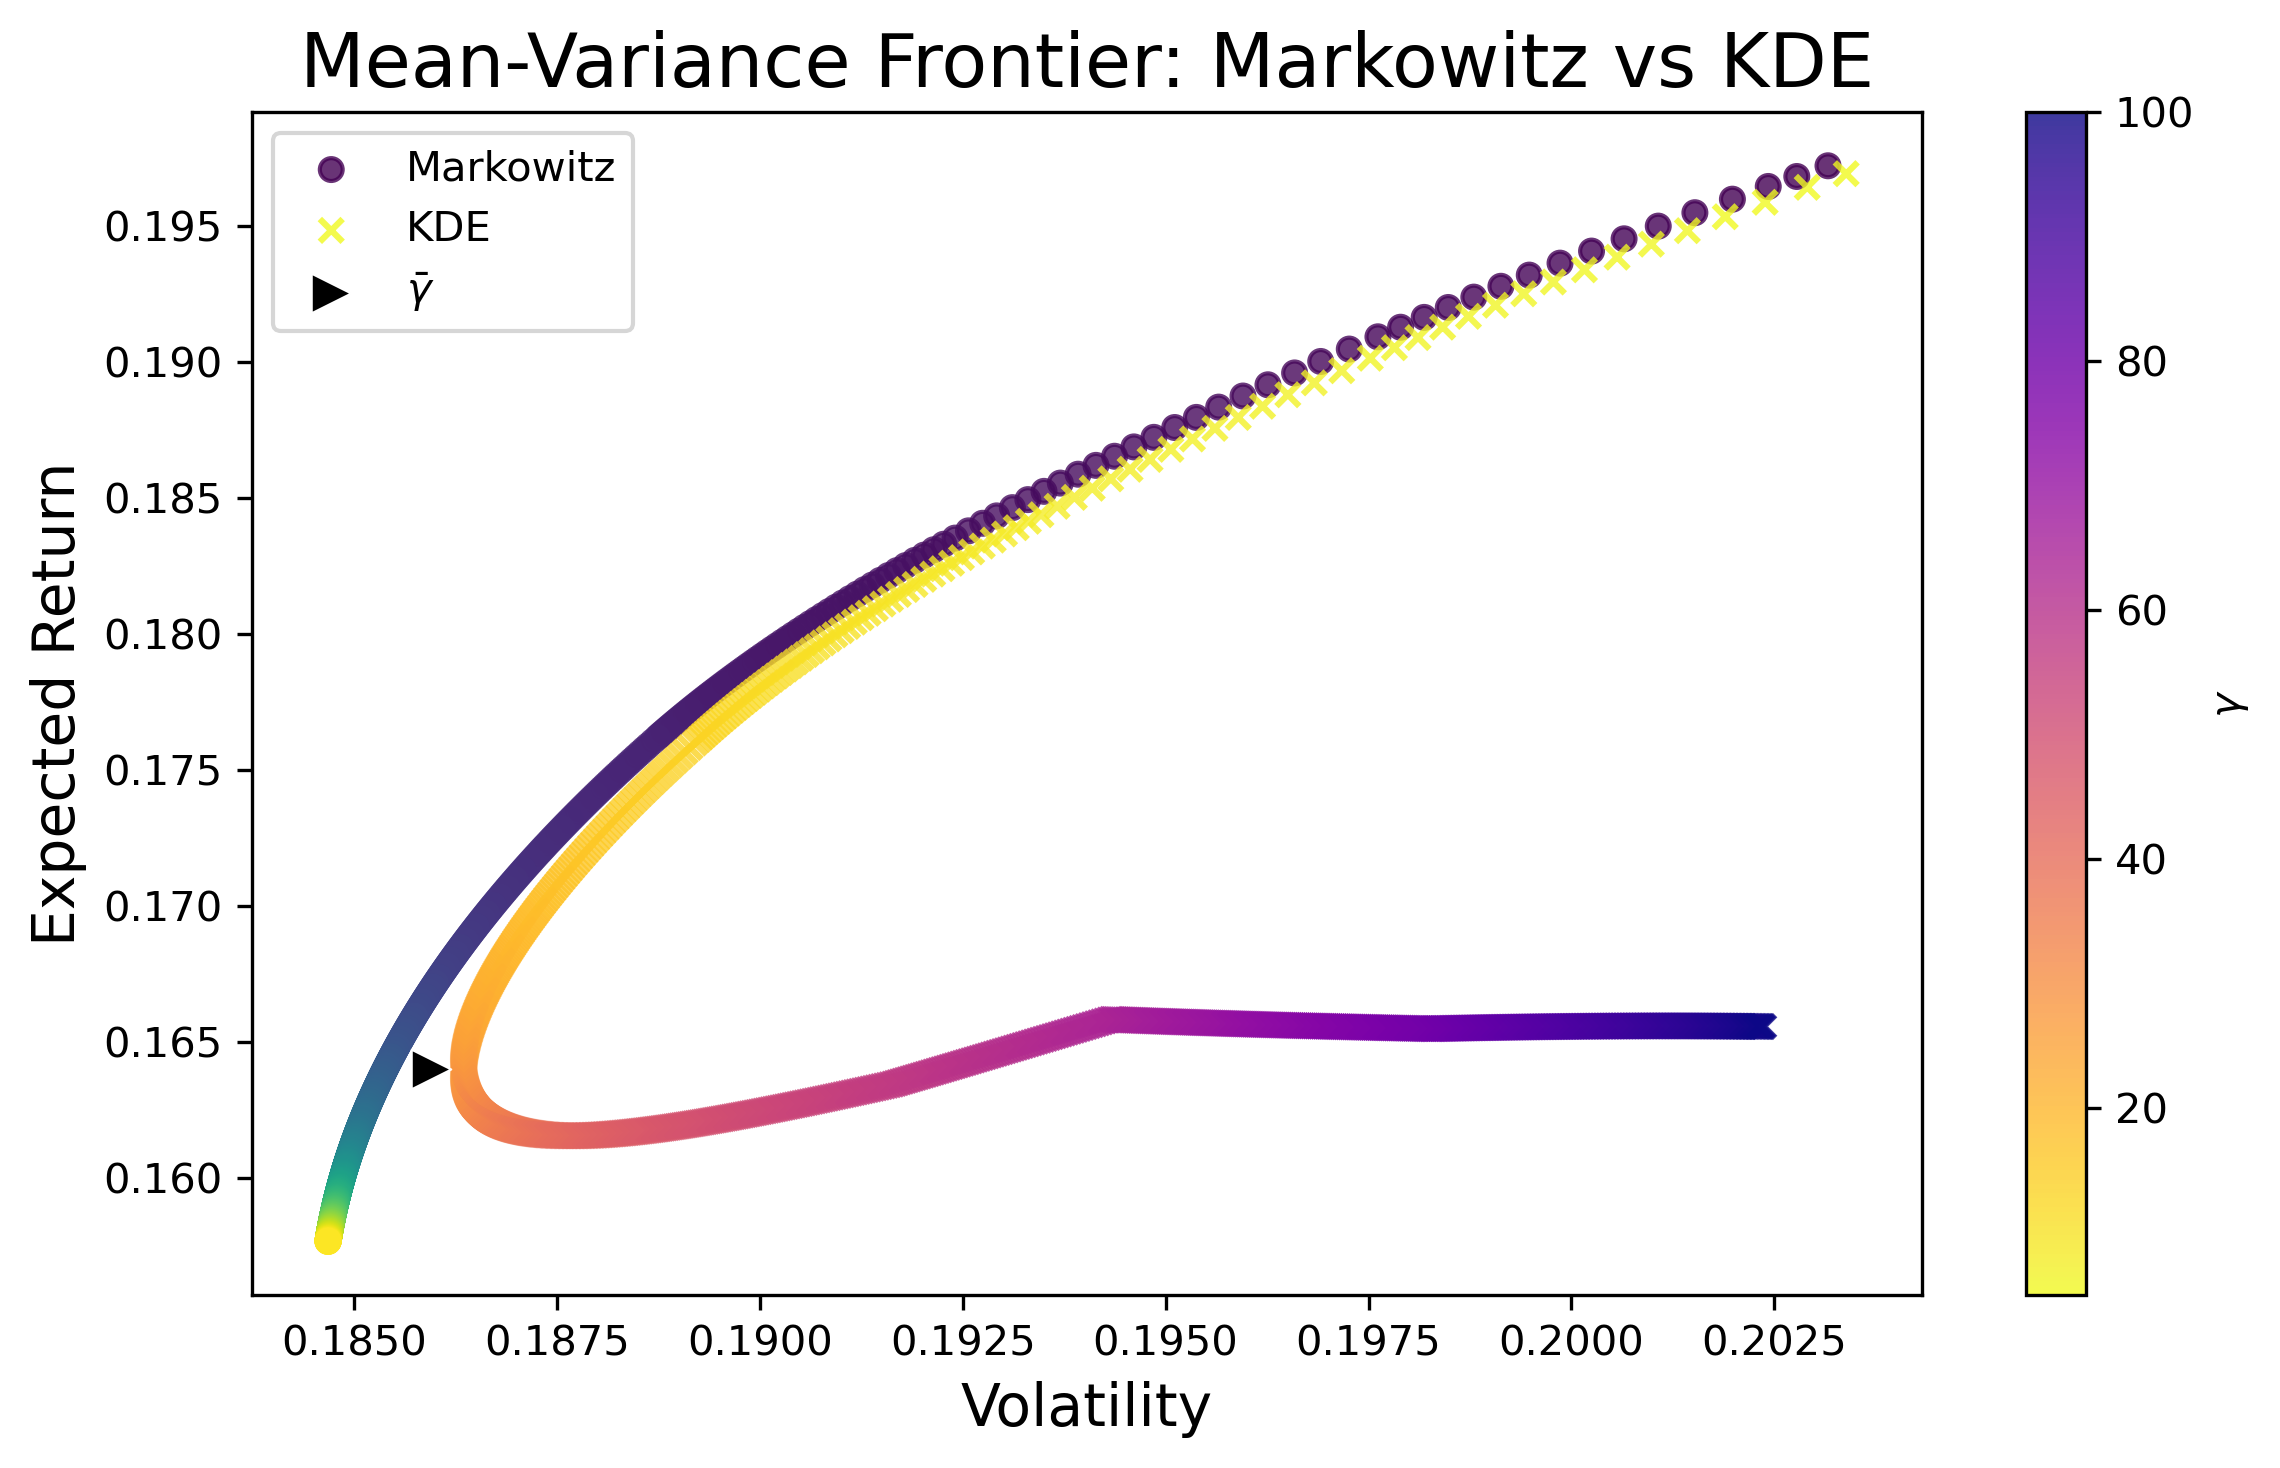
\includegraphics[width=\textwidth]{images/30_1.png}
    \end{minipage}
    \caption[Mean-variance frontier: Markowitz vs KDE]{Mean-variance efficient frontiers for risk-aversion parameters $\gamma\in[5,100]$, comparing classical Markowitz optimization (filled circles) with KDE-based optimization (crosses). Each marker is placed at the portfolio's expected volatility (x-axis) and expected return (y-axis) under a given $\gamma$, and colored from yellow (low risk aversion) to purple (high risk aversion). The $\blacktriangleright$ symbol indicates the minimum variance portfolio on the KDE frontier.}
    \label{fig:frontier1}
    \end{center}
    \end{figure}



This behavior contrasts with standard Markowitz optimization, where the highest risk aversion invariably results in the minimum variance portfolio. The KDE approach suggests a separation of two regimes of portfolio behavior, with a critical threshold value $\bar{\gamma}$. To better understand this phenomenon, we examine an alternative frontier situated in the risk-skewness space, rather than the risk-return space (using ex-post in-sample skewness). This second frontier shows that the apparent inefficiency in mean-variance space corresponds with improved skewness characteristics. 

\vspace{5mm}
\begin{figure}[H]
    \begin{center}
    \begin{minipage}{1\textwidth}
      \centering
      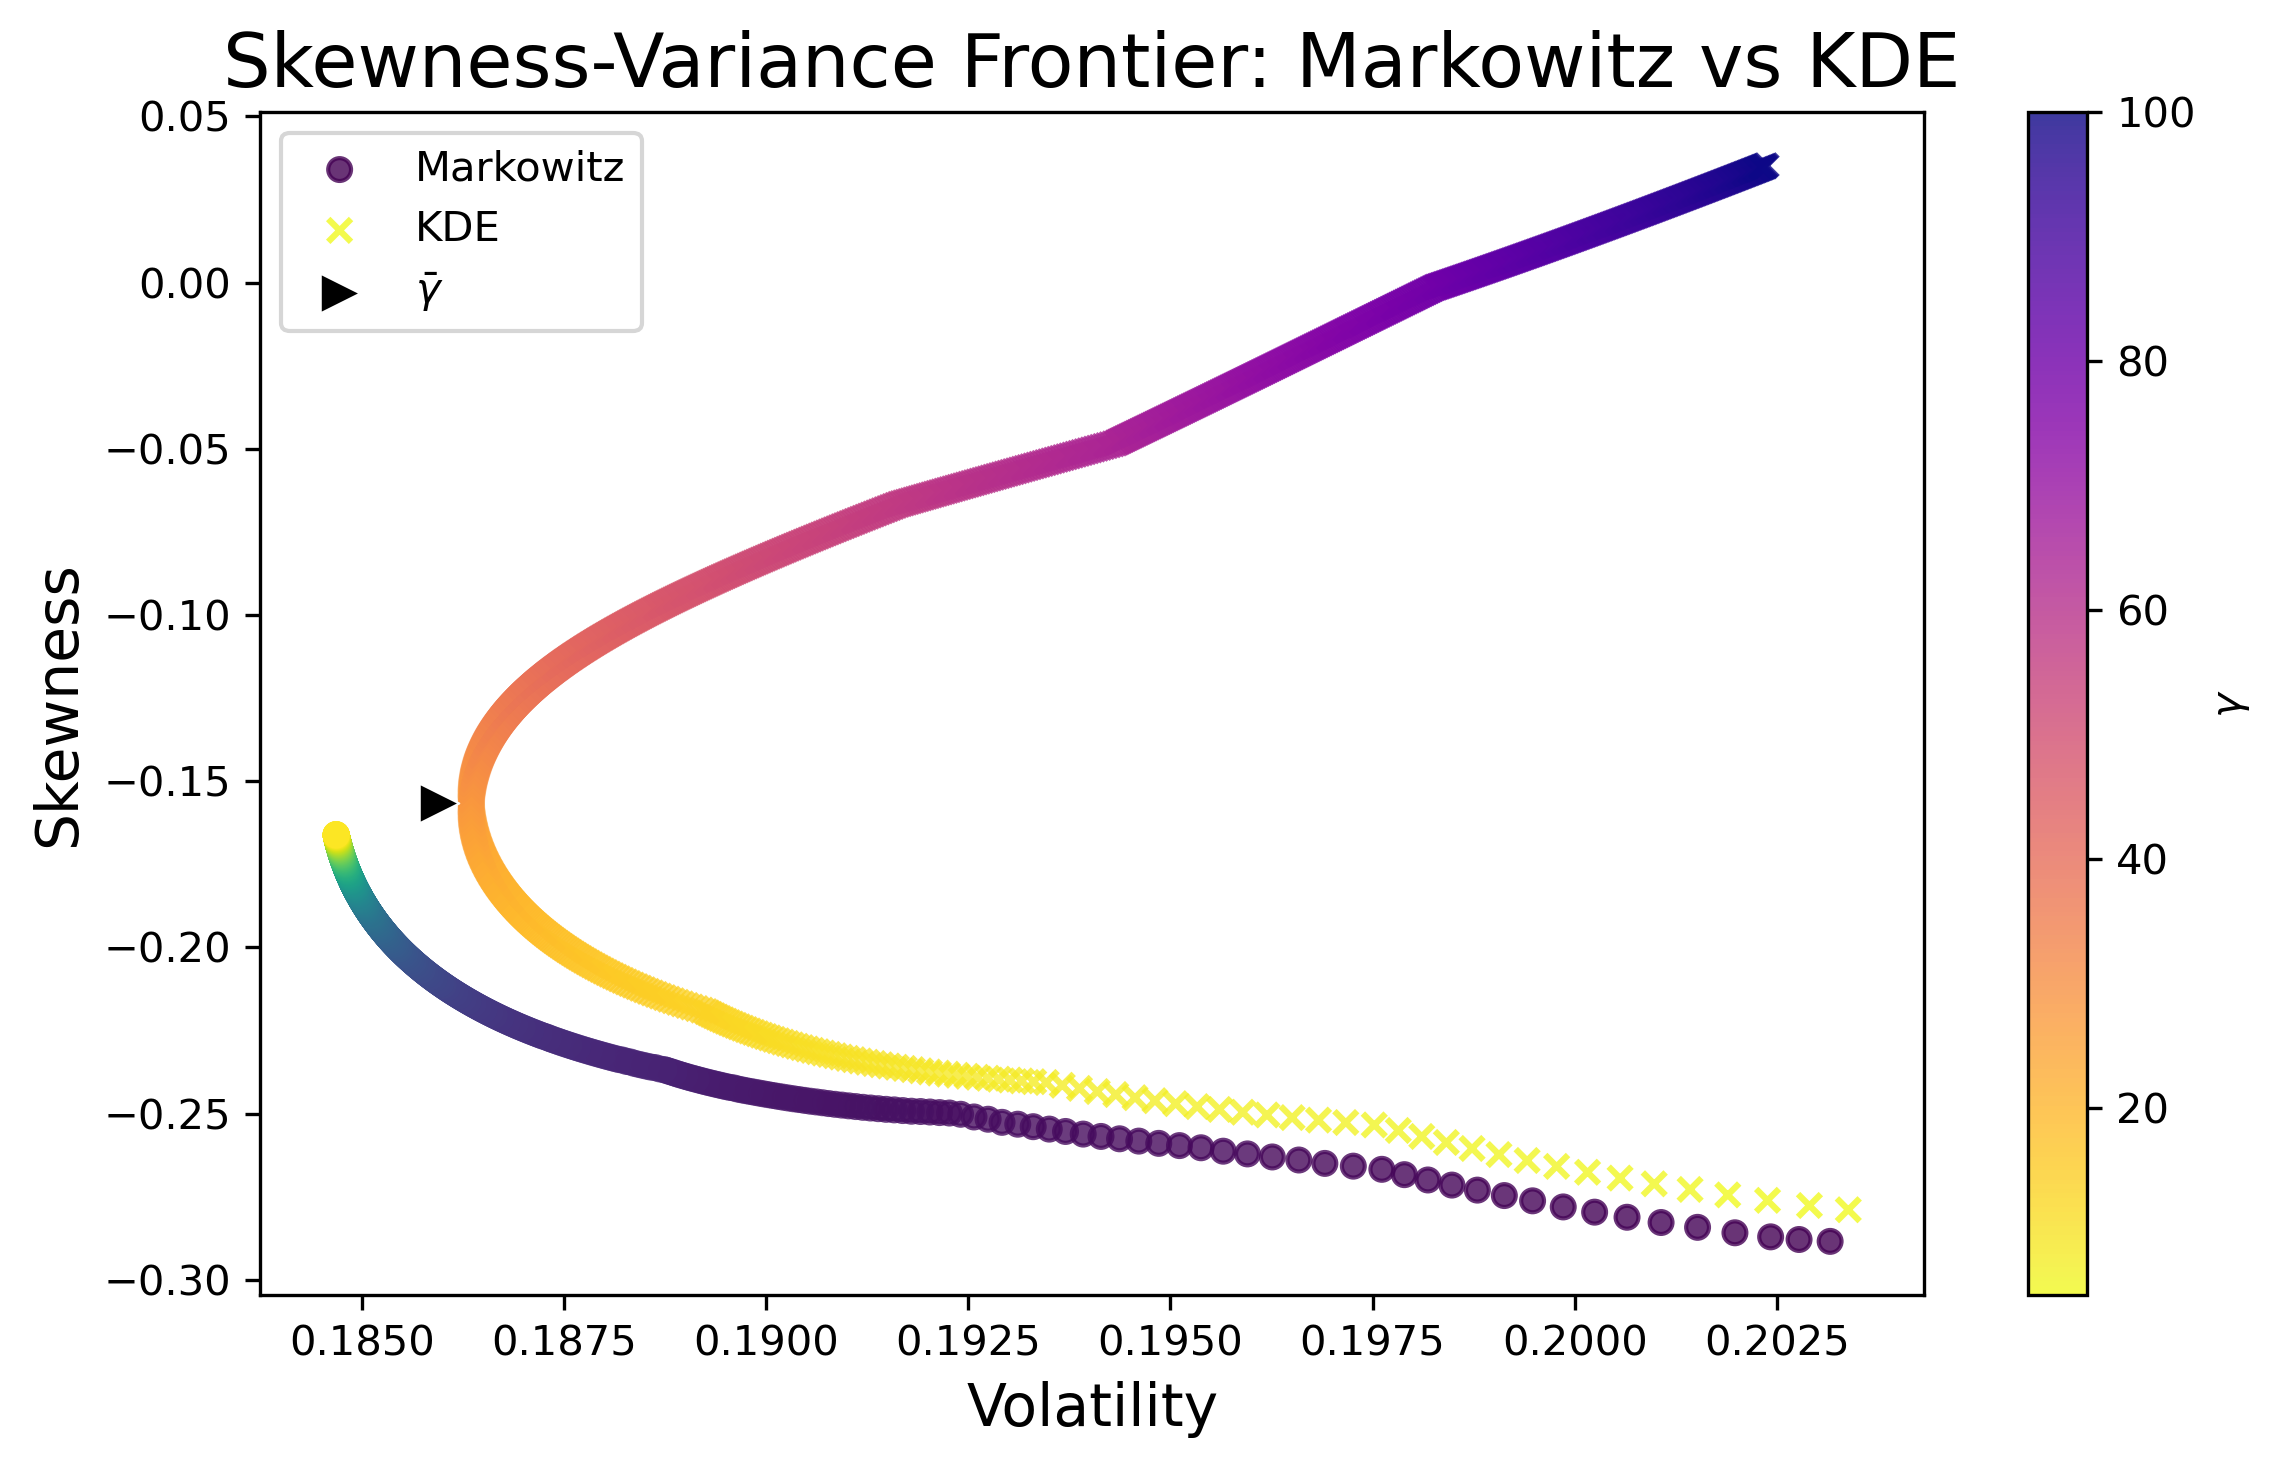
\includegraphics[width=0.65\textwidth]{images/30_2.png}
    \end{minipage}
    \caption[Skewness-variance frontier: Markowitz vs KDE]{Skewness-variance efficient frontiers. Here, the x-axis shows portfolio variance and the y-axis shows ex-post portfolio return skewness, with markers colored by $\gamma$ (yellow to purple). All other details are the same as in Figure \ref{fig:frontier1}.}

    \label{fig:frontier2}
    \end{center}
    \end{figure}

\newpage
As risk aversion increases, KDE initially approaches the Markowitz minimum variance portfolio but never reaches it. This occurs because the KDE optimization implicitly balances variance reduction against skewness improvement. At the point corresponding to $\bar{\gamma}$, the KDE minimum variance portfolio represents an equilibrium between these competing objectives, not a true global minimum in portfolio variance. Beyond this threshold, the priority for skewness improvement begins to dominate, causing the frontier to reverse direction along the volatility axis. This is the second reason why the volatility of the KDE minimum variance portfolio exceeds that of its Markowitz counterpart: it has already been implicitly incorporating skewness throughout the optimization process, compromising some variance reduction to achieve more favorable higher-moment characteristics.

Let us formally define a threshold of risk aversion $\bar{\gamma} > 0$ on the KDE mean-variance frontier corresponding to the KDE minimum-variance portfolio. Along the KDE frontier, all optimal portfolios with risk aversion $\gamma > \bar{\gamma}$ provide an inferior risk-return tradeoff compared to any portfolio with $\gamma \leq \bar{\gamma}$. Simultaneously, every portfolio in this dominated region exhibits higher skewness than any portfolio with $\gamma \leq \bar{\gamma}$. 

Thus, portfolios in the region where $\gamma > \bar{\gamma}$ simultaneously exhibit: (a) inferior mean-variance characteristics, and (b) superior variance-skewness attributes. This establishes a fundamental tension between competing criteria of portfolio efficiency and leads us to the following propositions:

\begin{proposition}\label{prop:skew-var}
Increasing the skewness of a portfolio beyond that of the minimum variance portfolio necessarily requires accepting a higher level of portfolio variance.
\end{proposition}

\begin{proposition}\label{prop:skew-sharpe}
Increasing the skewness of a portfolio beyond that of the minimum variance portfolio necessarily requires accepting a lower risk-return (mean-variance) profile than would have otherwise been attainable.
\end{proposition}

\begin{proposition}\label{prop:counterpoint}
Contrary to the prediction of the Markowitz framework, rational investors with the highest levels of risk aversion ($\gamma > \bar{\gamma}$) should not prefer the minimum variance portfolio, but should instead select portfolios with higher variance that offer improved skewness characteristics, thereby reducing exposure to extreme negative outcomes.
\end{proposition}

\subsection{Effect of H on KDE portfolios}
\label{sec:honkde}
Inspecting the effect of the variation in bandwidth on the KDE frontiers reveals a surprising result: the bandwidth parameter may be unimportant in the context of portfolio optimization. Figure \ref{fig:frontier3} demonstrates this by comparing efficient frontiers across multiple bandwidth scales.

\vspace{5mm}
\begin{figure}[H]
    \begin{center}
    \begin{minipage}{1\textwidth}
      \centering
      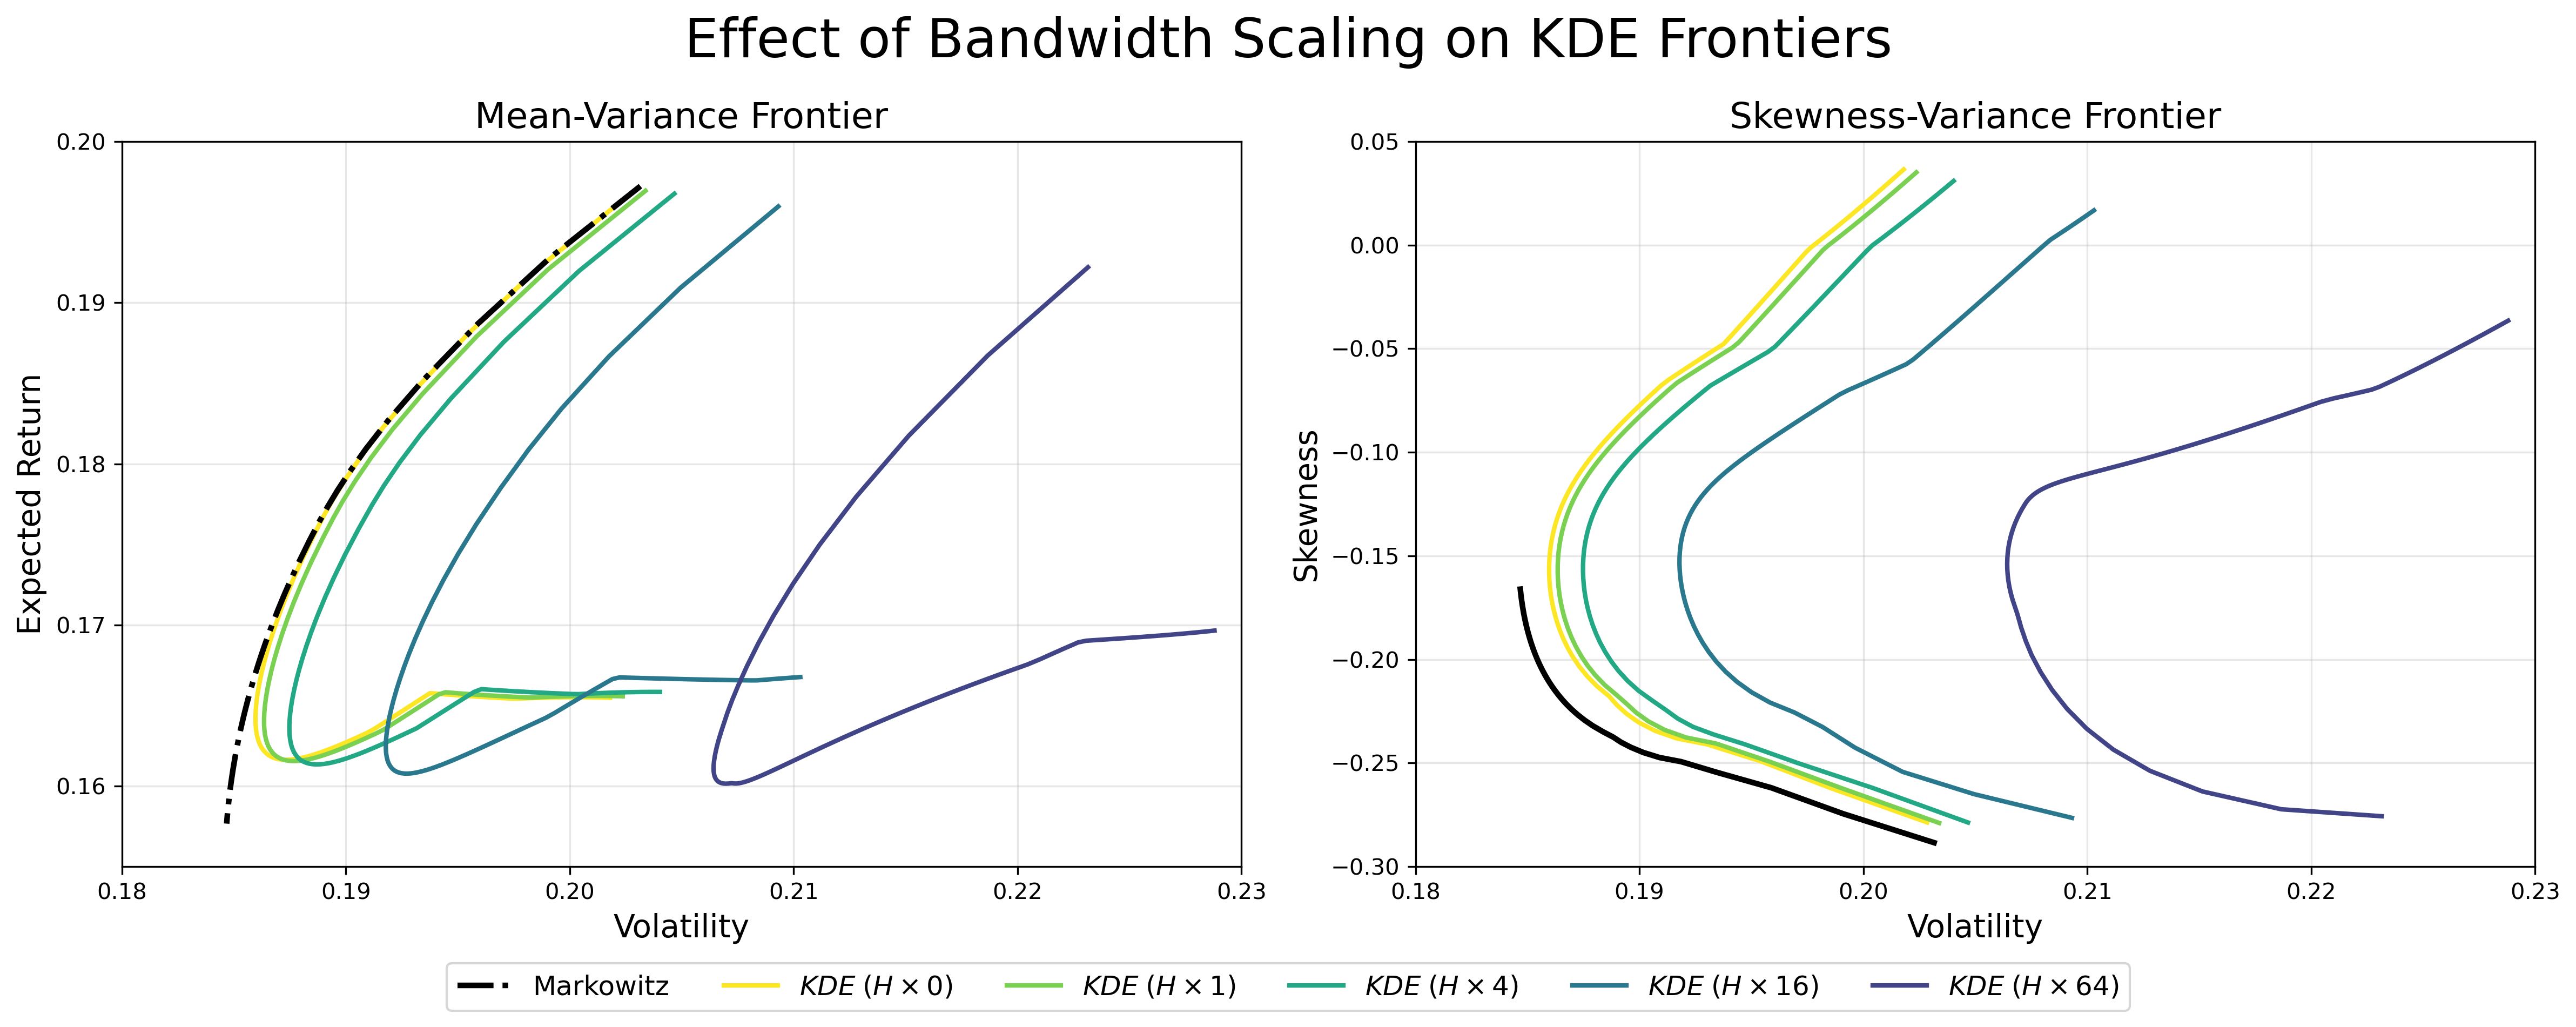
\includegraphics[width=\textwidth]{images/30_3.png}
    \end{minipage}
    \caption[Mean/Skewness-variance frontiers: KDE - Changing $H$]{Effect of bandwidth scaling on KDE-based efficient frontiers for $\gamma\in[5,100]$. \emph{Left:} Mean-variance frontier showing classical Markowitz (black dash-dotted) and KDE frontiers at $H\times\{0,1,4,16,64\}$ (colored solid lines, from light to dark). \emph{Right:} Corresponding skewness-variance frontier comparing the same curves, with skewness on the vertical axis. Increasing the bandwidth scale smooths the density estimate and shifts both frontiers, flattening the mean-variance curve and raising skewness at the cost of higher variance.}
    \label{fig:frontier3}
    \end{center}
    \end{figure}

In KDE, the quadratic term $\tfrac12\gamma^{2}\mathbf w^{\mathsf{T}}H\mathbf w$ sits inside the utility objective, while the ex-ante portfolio variance is $\sigma^{2}(\mathbf w)=\mathbf w^{\mathsf{T}}(H+\Sigma)\mathbf w$. Enlarging $h$ inflates both expressions, so for any fixed $\gamma$, the optimal variance $\sigma^{2}$ moves to the right. The shift is purely mechanical because a wider kernel leads to a stronger penalty on taking additional risk.

When $h=0$, the quadratic penalty disappears from the objective, and the low-$\gamma$ end of the KDE frontier coincides exactly with the Markowitz mean-variance frontier. More importantly, the entire $h=0$ frontier dominates all $h>0$ frontiers in variance-skew space, i.e., extra smoothing reduces improvements in skewness without delivering lower variance. This suggests that the bias-variance tradeoff logic of KDE does not translate into better portfolios.

Furthermore, $h$ and $\gamma$ are effectively substitutes. A larger $h$ lowers the critical risk aversion $\bar\gamma$ at which the KDE attains its lowest volatility. This is because a larger $H$ makes reductions in variance more costly, so a smaller increment in $\gamma$ switches the optimizer from variance-first to skewness-first. 

For the data set we study, the unsmoothed case $(H=0)$ already enables sensitivity to skewness through the adaptive weights $p_i$, and additional bandwidth appears only to reduce the effectiveness of this mechanism. Therefore, practitioners can consider skipping the bandwidth calibration step altogether. If bandwidth is removed from the objective function, KDE loses its interpretation as a tool for smoothing a discrete analytical function and becomes instead a convex backtest.

\subsection{Effect of K on GMM}
\label{sec:kongmm}
Figure \ref{fig:frontier4} presents efficient frontiers for GMM optimization across an increasing number of mixture components $K\in\{1,2,4,8,16\}$. The results reveal a more erratic pattern compared to the systematic behavior observed with KDE.

\vspace{5mm}
\begin{figure}[H]
    \begin{center}
    \begin{minipage}{1\textwidth}
      \centering
      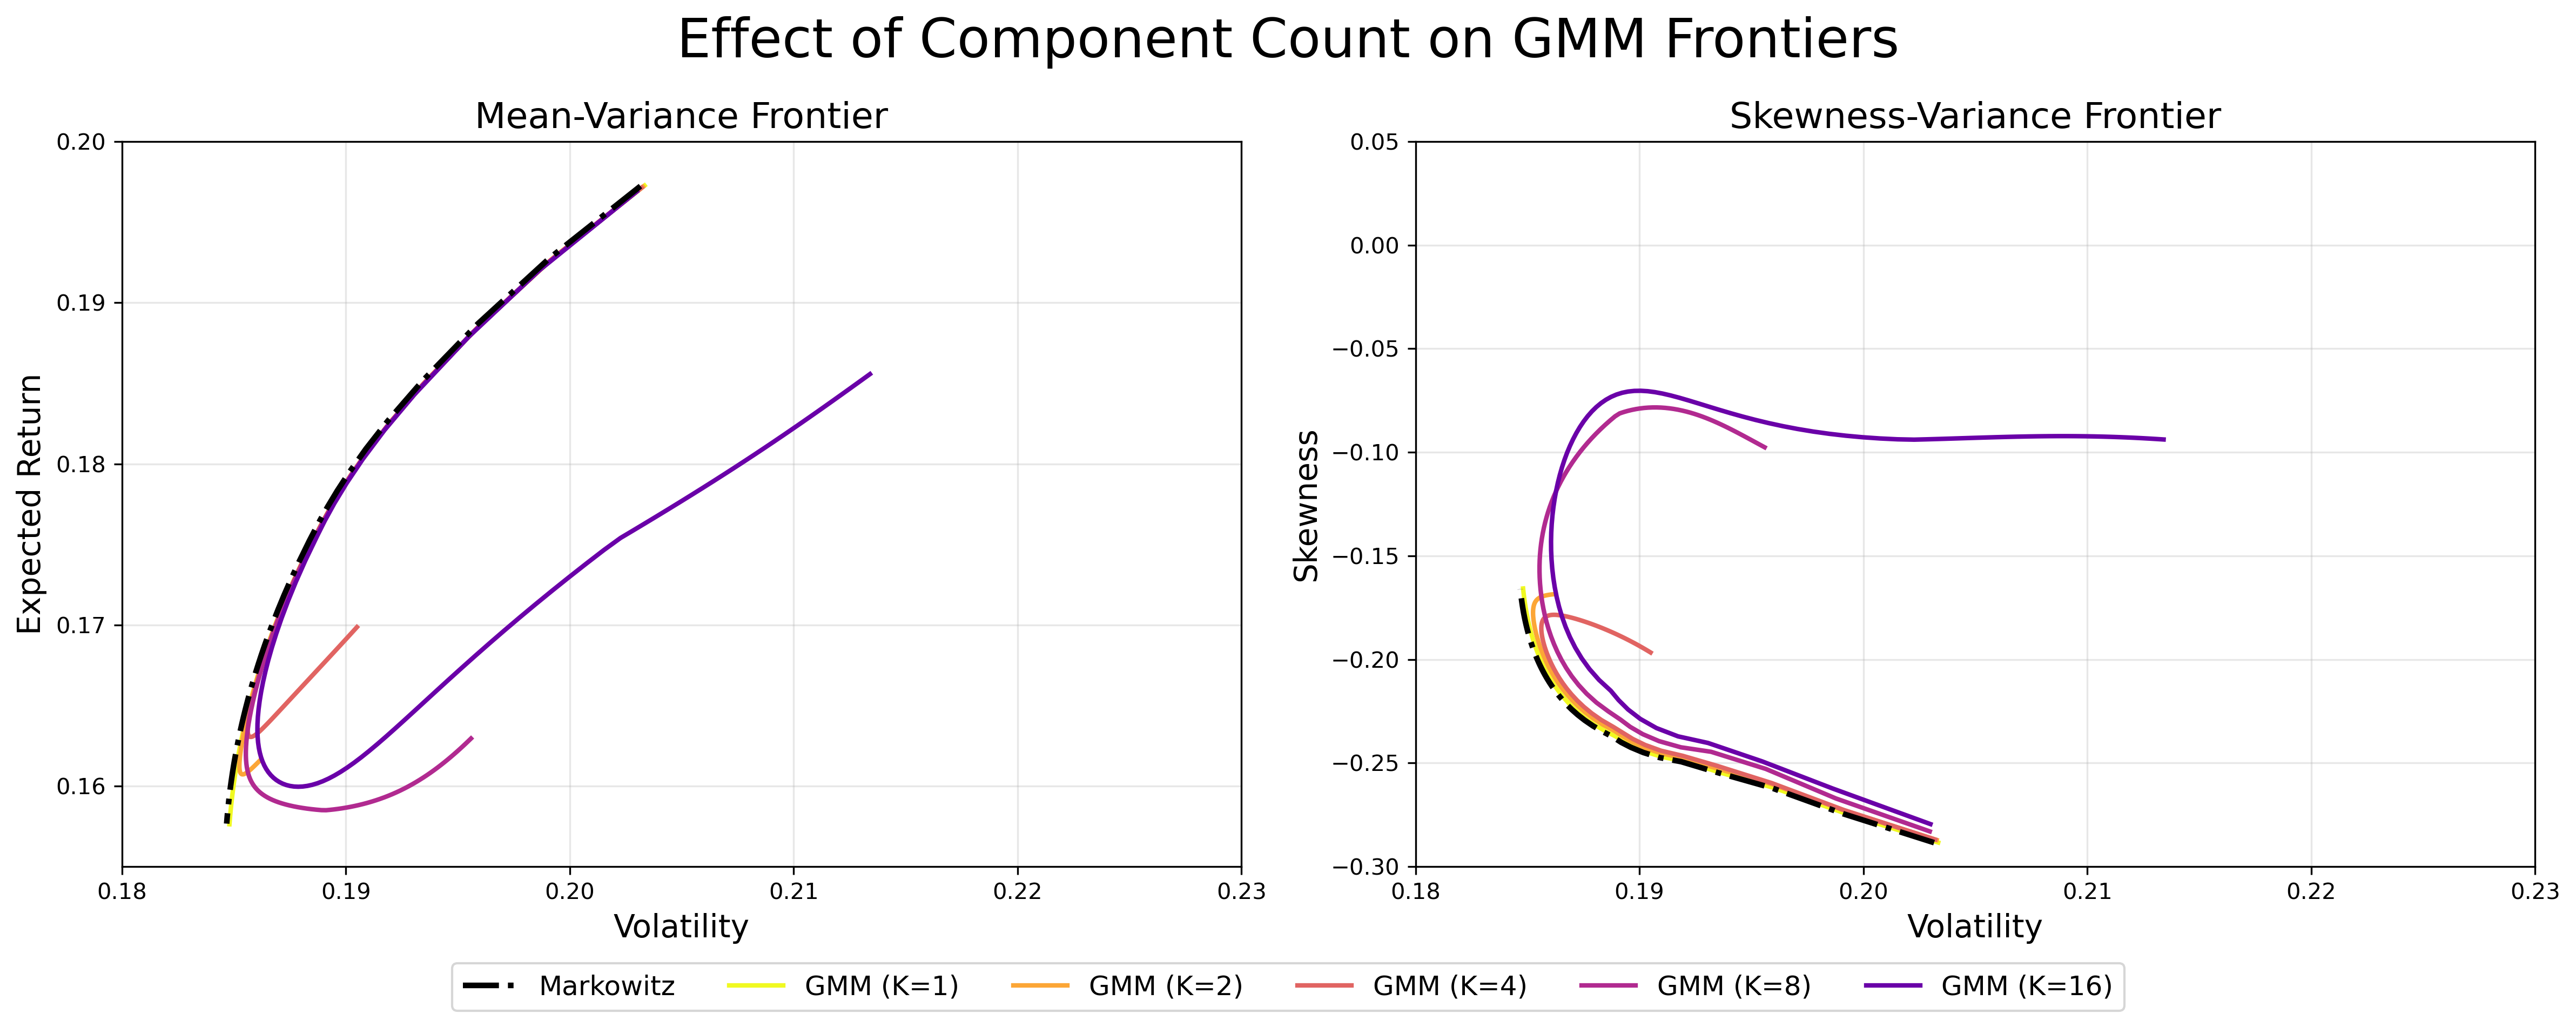
\includegraphics[width=\textwidth]{images/30_4.png}
    \end{minipage}
    \caption[Mean/Skewness-variance frontiers: GMM - Changing $K$]{Same format as Figure \ref{fig:frontier3}, but showing GMM efficient frontiers for varying numbers of mixture components $K\in\{1,2,4,8,16\}$. Figure bounds are unchanged.}
    \label{fig:frontier4}
    \end{center}
    \end{figure}

As expected, the $K=1$ frontier exactly reproduces the Markowitz frontier, representing a single multivariate normal distribution. Higher values of $K$ generate frontiers that qualitatively resemble KDE, with dominated regions in mean-variance space, where both expected return and volatility increase with risk aversion. However, the relationship between component count and frontier performance lacks the consistency observed with bandwidth scaling in KDE.

The $K=16$ frontier achieves the best mean-variance profile, with a steeper and more extended dominated region than other specifications. This steepness suggests that GMM potentially offers a superior return-volatility tradeoff. However, this advantage comes at a cost: all GMM frontiers substantially underperform KDE in the skew-variance space. Unlike KDE, where skewness continuously improves with increasing risk aversion, GMM frontiers tend to fold upon themselves, resulting in higher volatility and no skewness improvement beyond certain risk aversion levels.

These results suggest higher component counts are preferable. At the same time, increasing $K$ introduces significant computational complexity, especially for larger portfolios. With $K=16$ components potentially assigning a separate multivariate normal to each asset in our sample, GMM begins to resemble KDE conceptually, but with the crucial limitation of forcing individual assets into elliptical distributions.

\newpage
Thus, GMM occupies an awkward middle ground. It captures some non-normality benefits but lacks the ability to mitigate skewness like KDE. The inconsistent performance across different $K$ values, coupled with the computational requirements, makes GMM less attractive than either standard Markowitz (for simplicity) or KDE (for skewness improvement).

\subsection{Summary}
The frontier analysis demonstrates three key findings. First, KDE optimization establishes a clear tradeoff between mean-variance efficiency and skewness improvement, with portfolios beyond the critical risk aversion $\bar{\gamma}$ sacrificing mean-variance efficiency to achieve better skewness characteristics. Second, bandwidth selection in KDE appears largely inconsequential, with the unsmoothed case ($H=0$) delivering superior performance through its adaptive weighting mechanism alone. Third, GMM optimization shows inconsistent performance across different component counts and fails to match KDE's skewness improvements despite increased computational complexity. The empirical analysis that follows will examine how these theoretical properties translate into out-of-sample performance.